\chapter{Chi tiết Ontology Web Language}
\paragraph{Giới thiệu } - Như đã được đề cập trong phần cuối của chương trước, chức năng chính của OWL là một ngôn ngữ ontology cung cấp ngữ nghĩa cho Semantic Web. Trong nội dung chương này, chúng em sẽ giới thiệu về cú pháp, định dạng và chi tiết các đặc tính của ngôn ngữ Ontology Web. Phiên bản Ontology Web Language chúng em sử dụng là phiên bản 2 được tổ chức W3C khuyến khích sử dụng so với phiên bản OWL cũ 1.1 .
\section{Khái quát về OWL 2 \cite{owl2}}
\subsection{Tổng quan}
\begin{figure}[ht!]
	\centering
	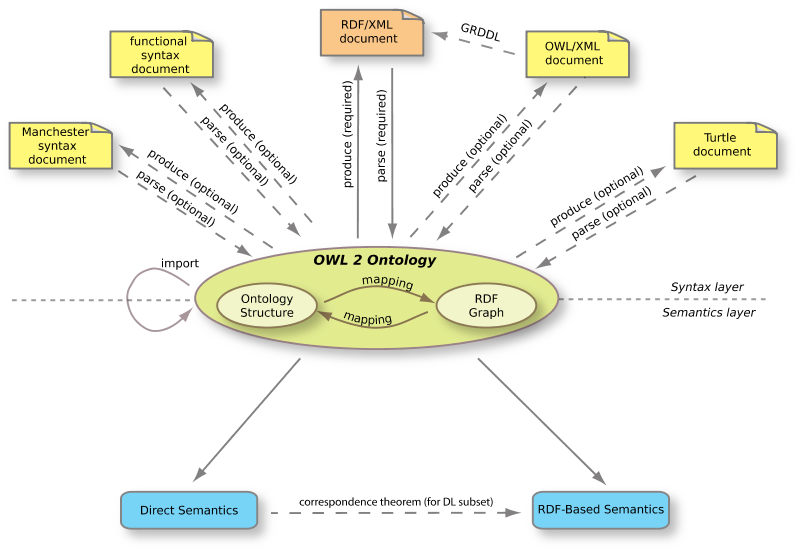
\includegraphics[width=120mm]{Figures/owl2structure.png}
	\caption{Cấu trúc của OWL 2\label{overflow}}
\end{figure}
Hình trên cho chúng ta cái nhìn tổng quan về các định dạng file, các loại cú pháp và cách khả năng serialization thành RDF Graph của Ontology. Như chúng ta thấy trong hình thì hình eclipse ở giữa thể hiện khái niệm trừu tượng của một ontology, có thể hiểu là một cấu trúc trừu tượng hay một đồ thi RDF. Chúng ta có thể dùng nhiều cú pháp để biểu diễn ontology và định dạng chúng dưới dạng file khác nhau (Syntex layer trong hình), các định dạng và cú pháp này hoàn toàn có thể chuyển đổi qua lại với nhau. Lớp ngữ nghĩa trong hình (semantic layer) cho thấy ngữ nghĩa được quy định theo 2 tiêu chuẩn kỹ thuật khác nhau là Direct Semantics và RDF-Based Semantics.
\\
Phần lớn những người phát triển Ontology bằng OWL2 sẽ chỉ cần 1 cú pháp (tương đương với 1 định dạng file) và một dạng biểu diễn ngữ nghĩa.
\subsection{Ontologies}
Bất kì ontology OWL2 nào đều có thể được định dạng như một đồ thị RDF. Mối quan hệ giữa 2 cách này được quy định bới cách tài liệu Mapping to RDF Graphs document [\href{http://www.w3.org/TR/owl2-overview/#ref-owl-2-rdf-mapping}{OWL 2 RDF Mapping}] \cite{mapping_rdf_graph}, trong tài liệu này định nghĩa rất rõ ràng một bảng map từ định dạng cấu trúc của ontology qua đồ thị RDF, và ngược lại. 
\subsection{Cú pháp}
Trong thực tế, một cú pháp cụ thể rất cần thiết để lưu trữ các OWL2 Ontologies và để trao đổi chúng giữa các công cụ và ứng dụng khác nhau. Cú pháp đầu tiên có khả năng hoán đổi là RDF/XML [\href{http://www.w3.org/TR/owl2-overview/#ref-rdf-syntax}{RDF Syntax}] \cite{rdfxml}. Ngoài RDF/XML có khả năng cung cấp khả năng tương tác giữ nhiều ứng dụng OWl2 khác nhau, các loại cú pháp khác đều có thể được sử dụng. Dưới đây là bảng so sánh và liệt kê các cú pháp.
\begin{table}[ht!]
\begin{tabular}{ |p{3cm}|p{4cm}|p{3cm}|p{4cm}|}
\hline
Tên cú pháp & Mô tả & Trạng thái & Mục đích sử dụng\\
\hline
RDF/XML & Mapping to RDF Graphs \cite{mapping_rdf_graph} \cite{rdfxml} & Bắt buộc & Hoán đổi được ( có thể viết và đọc được bằng nhiều phần mềm OWL2)
\\
\hline
OWL/XML & XML Serialization \cite{owlxml} & Tùy chọn & Xử lý dễ dàng hơn bằng công cụ XML.
\\
\hline
Functional Syntax & Structural Specification \cite{func_syntax} & Tùy chọn & Dễ đọc và hiểu được.
\\
\hline
Manchester Syntax & Manchester Syntax \cite{man_syntax} & Tùy chọn & Có ưu thế hơn để đọc/ghi DL Ontologies
\\
\hline
Turtle & Mapping to RDF Graphs \cite{mapping_rdf_graph} & Tùy chọn, không được công nhận chính thức & Có ưu thế để đọc/ghi RDF triples
\\
\hline
\end{tabular}
\caption{Bảng so sánh các cú pháp của OWL2\label{overflow}}
\end{table}
\subsection{Một số ví dụ của các syntax}
\subsubsection{Functional Syntax}
\begin{verbatim}
// Khai báo lớp
Declaration (Class (Animal)) l
Declaration (Class (Grass))) 
// Khai báo Object Property
Declaration (ObjectProperty (canEat))  
// Khai báo sub Class expression
SubClassOf (Cow Animal)  
// Khai báo sub Class Expression
SubClassOf (Cow ObjectSomeValueFrom(canEat Grass))  
\end{verbatim}
\subsubsection{RDF/XML Syntax}
\begin{verbatim}
T(Animal) rdf:type owl:Class
T(Grass) rdf:type owl:Class
T(canEat) rdf:type owl:ObjectProperty
T(Cow) rdfs:subClassOf T(Animal) 
T(Cow) rdfs:subClassOf T(_:x owl:someValuesFrom T(Grass))
\end{verbatim}
\subsubsection{OWL/XML Syntax}
\begin{verbatim}
<Declaration>
       <Class IRI="#Animal"/> // Khai báo lớp Animal
</Declaration>
<Declaration>
       <Class IRI="#Grass"/> // Khai báo lớp Grass
</Declaration>
<Declaration>
       <ObjectProperty IRI="#canEat"/> // Khai báo Object Property 
</Declaration>
<SubClassOf>
       <Class IRI="#Cow"/>
       <Class IRI="#Animal"/>  // Khai báo sub Class expression
</SubClassOf>
<SubClassOf>
       <Class IRI="#Cow"/>
<ObjectAllValuesFrom>
<ObjectProperty IRI="#canEat"/>  // Khai báo sub Class expression
       <Class IRI="#Grass"/>
</ObjectAllValuesFrom>
</SubClassOf>
\end{verbatim}
\subsubsection{Manchester Syntax}
\begin{verbatim}
Class: Cow 
    SubClassOf: Animal 
    SubClassOf: canEat some Grass
Class: Grass
ObjectProperty: canEat
\end{verbatim}
\section{Các đặc tính chi tiết của OWL2}
Ngôn ngữ Ontology Web Language 2 (hay OWL 2) đảm nhiệm chức năng thể hiện ngữ nghĩa cho Semantic Web như chúng ta đã thấy trong hình Semantic Web  Stack. OWL2 ontologies cung cấp các lớp (class), đặc tính (property), cá thể (individual) và các giá trị dữ liệu (data value), tất cả chúng sẽ được biểu diễn bằng các tài liệu và cú pháp được đề cập ở trên, phần này sẽ đi vào giải thích các thành phần vừa nêu ra của một ontology được viết bằng ngôn ngữ OWL2 . Đây cũng chính là các thành phần cấu trúc mà thư viện OWLAPI \cite{owlapi} áp dụng để xây dựng nên bộ thư viện giúp người phát triển ứng dụng ontology tương tác dễ dàng hơn với các tài liệu ontology.
Đầu tiên chúng em xin được giới thiệu tới đối tượng lớn nhất trong quy định của ngôn ngữ OWL2. 
\\
Tiếp theo, chúng em xin được trình bày về một qua các định nghĩa những thành phần cấu tạo của ontology mà có ảnh hướng đến quá trình xây dựng ứng dụng, các thành phần không liên quan sẽ không được đề cập.
\section{Định nghĩa các thành phần cấu tạo nên một ontology}
\subsection{Ontology IRI và Version IRI}
Mỗi ontology đều có thế có\textit{một ontology IRI\cite{iri}} (Internationalized Resource Identifier), dùng để định danh cho ontology. Nếu một ontology có một ontology IRI, thì ontology này có thể có thêm một version IRI, dùng để xác định phiên bản cho ontology này. Version IRI có thể trùng hoặc không cần thiết phải trùng với ontology IRI. Một ontology không có ontology IRI thì không có version IRI.
Dưới đây là những quy ước chọn ontology IRIs và version IRIs trong OWL2. Những đặc điểm kỹ thuật này không cung cấp cơ chế nào để làm chúng phải được tuân theo trên toàn hệ thống web. Tuy nghiên, những công cụ hay ứng dụng OWl2 \textit{nên} sử dụng những quy ước này để dễ dàng tìm ra lỗi trong những ontology mà chúng xử lý.
\begin{itemize}
\item Nếu một ontology có một ontology IRI nhưng không có version IRI, thì \textit{không nên tồn tại} một ontology với trùng ontology IRI vừa đặt.
\item Nếu một ontology có một ontology IRI và một version IRI, thì \textit{không nên tồn tai} một ontology khác với trùng ontology IRI và version IRI vừa đặt.
\item Tất cả các cách kết hợp khác của ontology IRI và version IRI không cần đòi hỏi tính duy nhất (unique). Như vậy 2 ontologies khác nhau có thể không có ontology IRI và version IRI; tương tự, một ontology chưa một ontology IRI có thể cùng tồn tại cùng với một ontology khác có cùng ontology IRI vừa đặt \textbf{và} các version IRI của các ontologies này \textbf{phải} khác nhau.
\end{itemize}
Ontology IRI và các version IRI kết hợp với nhau giúp định danh một phiên bản cụ thể của của ontology từ một bộ chưa tất cả các phiên bản của một ontology cụ thể nào đó được định danh chung bằng ontology IRI. Trong mỗi bộ ontology như vậy, sẽ có chính xác một ontology được dùng nhưng một ontology hiện hành - khi dùng ontology IRI để truy vấn ontology mà không đề cập version IRI mặc định ontology co verison IRI hiện hành sẽ được trả về.

%\subsubsection{Tài liệu Ontology}
%Bản chất OWL 2 Ontology chỉ là một khái niệm trừu tượng chiếu theo định nghĩa trong các đặc tính cấu tạo của nó, để biểu diễn những ngữ nghĩa trong ontology và lưu trữ chúng, chúng ta cần một dạng tài liệu được quy ước. Cụm từ "Tài liệu ontology" (\textit{Ontology Document}) muốn nói đến khả năng một số lượng lớn ontologies có thể được lưu giữ trong một tài liệu thực sự được biểu diễn dưới dạng một trong các cú pháp vừa nếu ở phần. 

\subsection{Thực thể, trực nghĩa và cá thể ẩn danh - Entities, Literals and Anonymous Individuals}
Các thực thể (entities) là thành phần cơ bản nhất của OWL2 Ontology, chúng định nghĩa các từ vừng - cụ thể là những đặt tên ra các khái niệm (named term) - của một ontology. Bên cạnh các thực thể, OWL 2 ontologies thường có thêm các trực nghĩa (literals), như strings hay integers.
\begin{figure}[ht!]
	\centering
	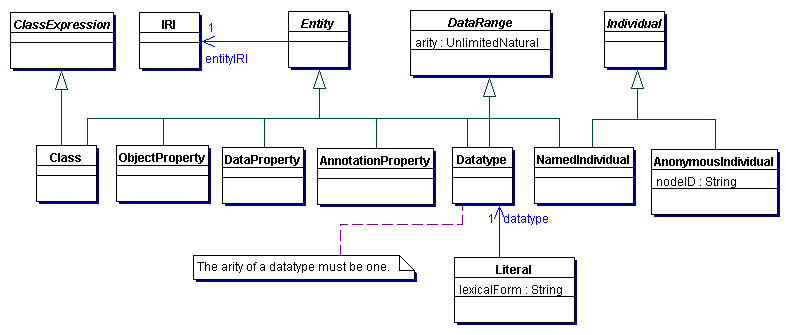
\includegraphics[width=140mm]{Figures/entities.png}
	\caption{Entities, Literals, Anonymous Individuals trong OWL2 \label{overflow}}
\end{figure}
\\
Cấu trúc của các thực thể và trực nghĩa trong OWL 2 được thể hiện trong hình bên. Các lớp (classes), kiểu dữ liệu (datatypes), đặc tính đối tượng (object properties), đặc tính dữ liệu (data properties), thuộc tính chú thích và các cá thể có tên đều được gọi chung là các thực thể (entities), tất cả chúng được được định danh bằng một IRI duy nhất. 
\begin{itemize}
\item Lớp (class) đại diện cho một tập gồm nhiều cá thể(individuals).
\item Kiểu dữ liệu (datatype) là một tập của các trực nghĩa như strings hoặc integers.
\item Đặc tính đối tượng và dữ liệu (object \& data property) được sử dũng để biểu diễn các mối quan hệ giữa các cá thể với cá thể khác và giữa cá thể với kiểu dữ liệu trong một miền (domain) nào đó.
\item Đặc tính chú thích (annotation) được dùng để đưa thêm những thông tin không có tính ngữ nghĩa( non-logical) như các chú thích, giải nghĩa, ngôn ngữ gắn với ontologies, các phát biểu/ tiên đề (axioms) và các thực thể.
\item  Các cá thể có tên có thể được dụng để biểu diễn một đối tượng cụ thể từ một lớp nào đó.
\end{itemize}
Bên cạnh các cá thể có tên, OWL2 còn cung cấp một khái niệm gọi là các cá thể ẩn danh (anonymous individuals) - là cá thể tương tự với các node trống (blank nodes) trong RDF Concept \cite{rdf_concept} và được truy xuất ngay bên trong ontology mà chúng được sử dụng. Cuối cùng, OWL 2 cung cấp thêm cho cac trực nghĩa (literals), một dạng dữ liệu string gọi là định dạng nghĩa bằng từ ngữ (lexical form) và một dạng dữ liệu để chỉ dẫn cách ontology có thể hiểu chuỗi này.
% Classes 
\subsubsection{Lớp (Classes)}
Lớp được hiểu như tập hợp các cá thể. Hai lớp với IRIs \textit{owl:Nothing} và \textit{owl:Thing} là các lớp được định nghĩa sẵn trong OWL2 với ý nghĩa như sau:
\begin{itemize}
\item \textbf{owl:Thing} là tập hợp gồm tất cả các cá thể.
\item \textbf{owl:Nothing} là tập hợp rỗng,
\end{itemize}
Không nên sử dụng 2 định nghĩa trên để gán cho bất kì lớp nào trong OWL 2 DL Ontology.
% Datatypes
\subsubsection{Kiểu dữ liệu (datatypes)}
Kiểu dữ liệu là thực thể được xem như tập hợp của các giá trị dữ liệu. Như vậy, kiểu dữ lữ liệu cũng tương tự lớp, khác biệt chính là thay vì chứa các cá thể (individuals) như lớp thì lại chứ các giá trị dữ liệu như strings, numbers, Kiểu dữ liệu có thể được dùng tạo ra các dữ liệu giới hạn (datarange).
\\
Ví dụ:
\\
Kiểu dữ liệu \textit{xsd:positiveInteger} đại diện cho tập hợp gồm tất cả các số nguyên dương. Nó được sử dụng để quy định kiểu dữ liệu mà đặc tính \textit{hasAge} có thể chấp nhận.
\begin{verbatim}
DataPropertyRange( a:hasAge xsd:positiveInteger) 
// đặc tính dữ liệu a:hasAge chỉ được phép là các số nguyên dương.
\end{verbatim}
% Object Properties
\subsubsection{Đặc tính đối tượng (object properties)} 
Đặc tính đối tượng kết nối các cặp cá thể - tạo ra mối liên hệ (relationship) giữa các cá thể. Tương tự lớp cũng có 2 đặc tính đối tượng được định nghĩa sẵn trong OWL 2 với ý nghĩa như sau:
\begin{itemize}
\item \textbf{owl:topObjectProperty} kết nối tất cả các cặp cá thể có thể kết nối.
\item \textbf{owl:bottomObjectProperty} không kết nối bất kì cặp cá thể nào. 
\end{itemize}
Cũng không nên sử dụng 2 định nghĩa trên để gán cho bất kỳ đặc tính đối tượng nào trong OWL 2 DL Ontology. Đặc tính đối tượng \textit{a:parentOf} được dùng để nói lên mối quan hệ giữ các cá thể. Nó có thể được sử dụng như trong phát biểu sau:
\begin{verbatim}
ObjectPropertyAssertion( a:parentOf a:Peter a:Chris)  
\end{verbatim}
\textbf{Giải thích:} Peter là ba mẹ của Chris.

% Data Properties
\subsubsection{Đặc tính dữ liệu (data properties)}
Đặc tính dữ liệu liên kết các cá thể với các trực nghĩa. Trong một vài hệ thống biểu diễn tri thức, đặc tính dữ liệu chức năng được gọi là thuộc tính.
Hai định nghĩa sẵn \textit{owl:topDataProperty} và \textit{owl:bottomDataProperty} có ý nghĩa như sau
\begin{itemize}
\item \textbf{owl:topDataProperty} liên kết tất cả cá thể với tất cả các trực nghĩa.
\item \textbf{owl:bottomDataProperty} không liên kết bất kì cá thể với trực nghĩa nào.
\end{itemize}
Tương tự lớp và đặc tính đối tượng, 2 phát biểu \textit{top} và \textit{bottom} trên cũng không nên được sử dụng để gán cho bất kì đặc tính dữ liệu nào. Mỗi đặc tính dữ liệu \textit{a:hasName} chứa tên đầy đủ của mỗi người. Ví dụ nó có thể được sử dụng như trong phát biểu sau:
\begin{verbatim}
DataPropertyAssertion( a:hasName a:Steve "Steve Job") 
\end{verbatim}
\textbf{Giải thích:} Tên của Steve là "Steve Job".

% Individuals
\subsubsection{Cá thể (Individuals)}
Cá thể trong OWL2 là một đối tượng cụ thể thuộc một tập/lớp (domain/class). Có 2 dạng cá thể trong cú pháp OWL2. \textit{Cá thể có tên} được khai báo tên một cách rõ ràng để có thể sử dụng trong bất kì ontology nào bằng cách truy vấn tới IRI có chứa tên của nó. Ngược lại, cá thể ẩn danh (Anonymous Individuals) không có tên gọi toàn cục và chỉ truy vấn được trong nội bộ của ontology chứa chúng.

% Named Individuals
\paragraph{Cá thể có tên (Named Individuals)} được định danh bằng một IRI. Vì vậy, nên cá thể có tên cũng là một thực thể (entity) tương tự lớp, đặc tính và kiểu dữ liệu. Ví dụ khai báo một các thể thuộc 1 lớp:
\begin{verbatim}
ClassAssertion( a:Person a:Peter)
\end{verbatim}
\textit{Giải thích:} Peter là một người.

% Anonymous Individuals
\paragraph{Cá thể ẩn danh (Anonymous Individuals)} Nếu cần một cá thể chỉ sử dụng ở nội bộ ontology, chúng ta có thể sử dụng cá thể ẩn danh, được định danh bằng một node ID cục bộ thay vì sử dụng IRI toàn cục. Cá thể ẩn danh tương tự như một node rỗng trong đồ thị RDF \cite{rdf_concept}. Ví dụ khai báo đặc tính đối tượng giữa cá thể ẩn danh với cá thể có tên:
\begin{verbatim}
ObjectPropertyAssertion( a:liveAt a:Peter _:a1)
ObjectPropertyAssertion( a:city _:a1 a:HCM)
ObjectPropertyAssertion( a:district _:a1 a:ThuDuc)
\end{verbatim}
\textbf{Giải thích:} Peter sống ở một địa chỉ nào đó (chưa biết). Mà địa chỉ chưa biết này nằm trong thành phố Hồ Chí Minh và nằm trong quận Thủ Đức.



